\section{Introduction}

%%%%%%%%%%%%%%%%%%%%%%%%%%%%%%%%%%%%%%%%%%%%%%%%%%%%%%%%%%%%%%%%%%%%%%%%%% Problem definition
% Motivation of research domain
Recent advances in hardware technology have led to the production of consumer appropriate head mounted displays (HMDs) such as the Oculus Rift (the Oculus), ideal for personal use in immersive Virtual Reality (VR) applications including gaming, simulation, and film. Support from established companies such as Valve Software~\cite{valveVR} and the availability of the Oculus source development kit has resulted in a heretofore unseen, rapidly expanding ecosystem of applications, games and movies specifically designed for VR. This, coupled with the high quality and low price of the Oculus represents the first time VR has been so widely accessible in the market. \\

% What is the main issues of the research domain ?
Although HMDs represent an ideal set-up for immersive viewing of 3D stereoscopic content, they have a significant downside; people commonly report adverse physical reactions when using HMDs. These reactions include discomfort symptoms such as headaches, nausea, dizziness and eye-strain~\cite{howard02}, comparable to the symptoms commonly reported by sufferers of motion sickness. Collectively, these symptoms represent a condition referred to as \textbf{\textit{simulator sickness}}~\cite{mccauley84}. We refer to \textbf{\textit{visual discomfort}} as the specific subset of simulator sickness symptoms caused by visual stimuli. It has been found that up to 80\% of people experience these adverse reactions when using HMDs~\cite{Stanney03}.\\

% Why are they important and what is challenges ?
The human visual system uses a number of cues to infer depth and distance. Foremost among these cues are accommodation, the flexion of the lens in the eye required to form a focused image on the retina, and vergence, the inward rotation of the eyes required to form a single, binocular image. In stereo displays, these cues do not match, as the accommodation required to bring the physical HMD screen into focus will rarely match the vergence required to fuse the stereo image pair into a single binocular image, as shown in Fig.~\ref{fig:av-conflict}. This is caused by the requirement that the eyes converge to a variety of different depths, depending on the virtual depth of the observed object in the stereoscopic scene~\cite{rushton99}. The result of this mismatch is a conflict in the expected depths of visual stimuli, which is known to be a cause of visual discomfort~\cite{shibata11}. In stereoscopic 3D viewing, if the accommodative demand is fixed (as is the case for HMDs such as the Oculus) and a change in vergence demand occurs, a greater rate of change in the vergence demand will result in greater visual discomfort~\cite{kim14}. This indicates that it is not just the existence of conflict between accommodation and vergence demands that leads to discomfort: the requirement for the visual system to consistently re-adapt to new, conflicting demands is also a factor.\\ 

\begin{figure}
        \centering
            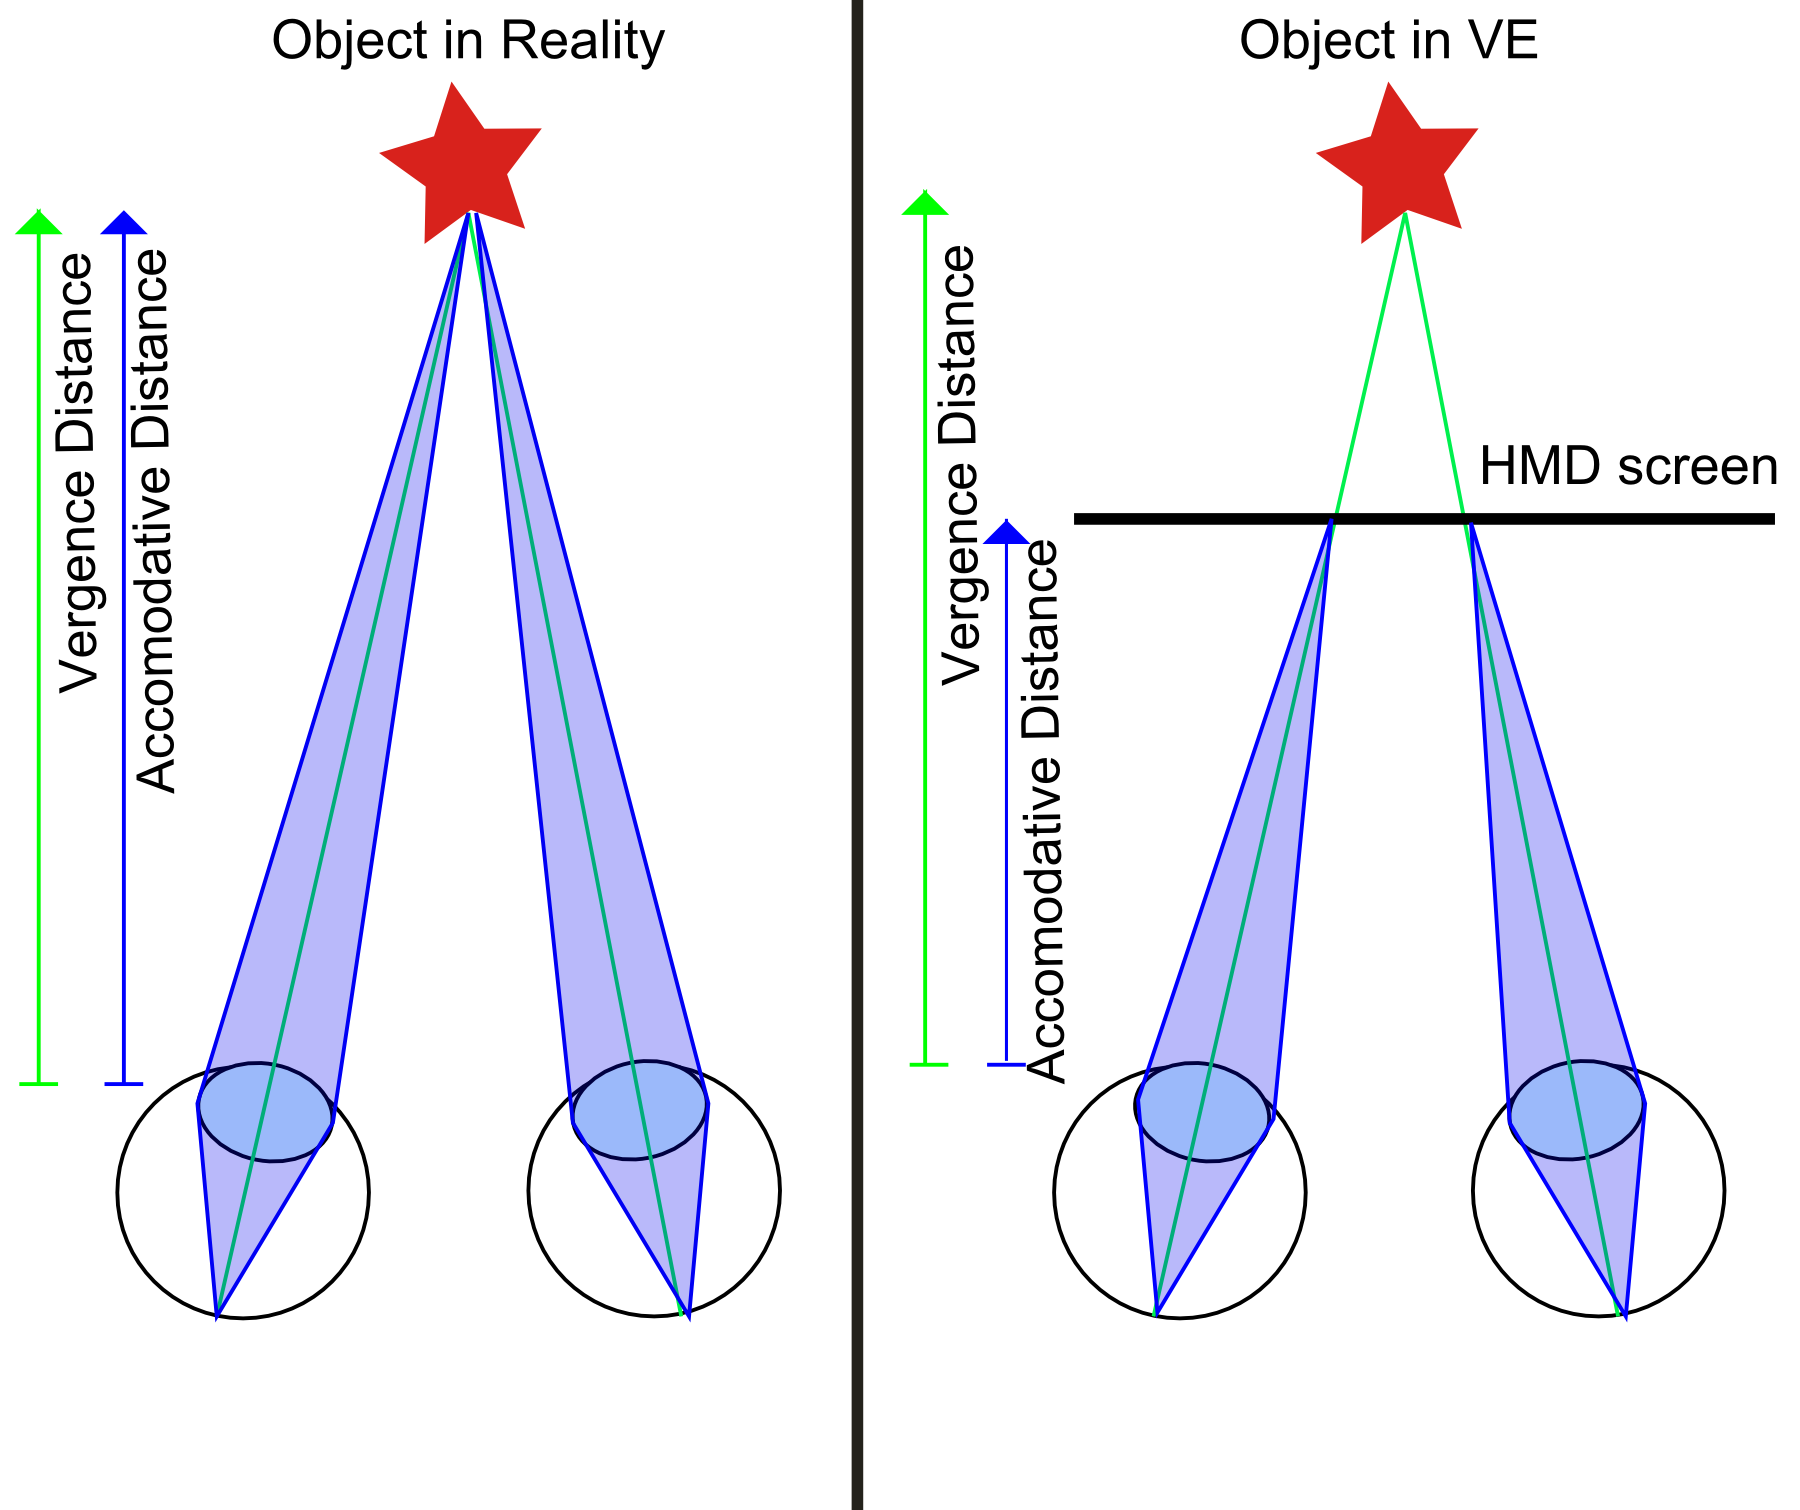
\includegraphics[width=0.45\textwidth]{images/vaconflict.png}
            \caption{An illustration of the accommodation-vergence conflict: comparing visual situations in real life (left) and when seeing objects in virtual environment (VE) on a HMD (right)}
            \label{fig:av-conflict}
\end{figure}

% Why is it challenging or What is the limitation of the previous work ?
%Moss and Muth\cite{moss08} report that modification to HMD hardware designed is required to reduces Visual Discomfort, a suggestion implementations such as Lanman and Luebke's\cite{Lanman13} light field display HMD follow. 
Following the suggestion that modifications to HMD hardware are required to reduce visual discomfort~\cite{moss08}, new hardware solutions such as the light field display HMD~\cite{lanman13} have been proposed. These implementations show promising results in reducing discomfort, but still have practical limitations including low display resolutions and pixel pitches. Gaze-contingent DoF can reduce visual discomfort when viewing stereoscopic content on LCD monitors viewed through a haploscope, according to a recent perceptual study~\cite{duchowski14}. This study used an external eye-tracking system to provide accurate calculation of participants gazes when using the haploscope. The requirement for such external hardware is intrusive in psychophysical evaluations of consumer level devices and may not accurately represent viewing conditions for users outside the lab. \\


In this paper, we perceptually evaluate the human visual system to show the effectiveness of dynamic DoF blur in mitigating visual discomfort when using stereoscopic HMDs. As far as we know, this is the first experimental report to investigate the effectiveness of dynamic DoF blur on HMDs. Our test system can be realised without any hardware modification and requires no usage of intrusive external devices: it relies only on positional data already captured by the Oculus. We implement a real-time dynamic DoF system in the Unreal Engine (Version 4)~\cite{unreal} and perform a series of psychophysical tests to show the effectiveness of the dynamic DoF blur on the Oculus. We use participant responses to questions about their subjective levels of discomfort as a metric, using a questionnaire based off the \say{Simulator Sickness Questionnaire (SSQ)}~\cite{kennedy93}. \\

\begin{figure*}
        \centering
            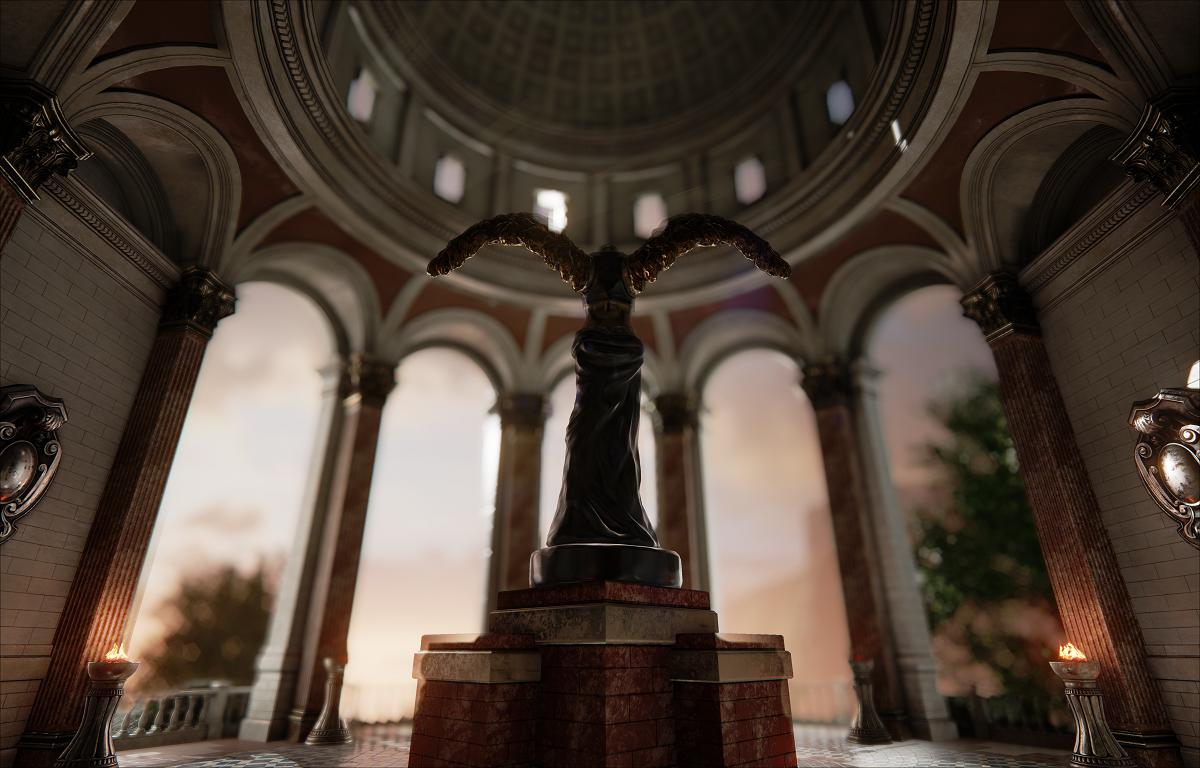
\includegraphics[width=0.45\textwidth]{images/lighton.png}
            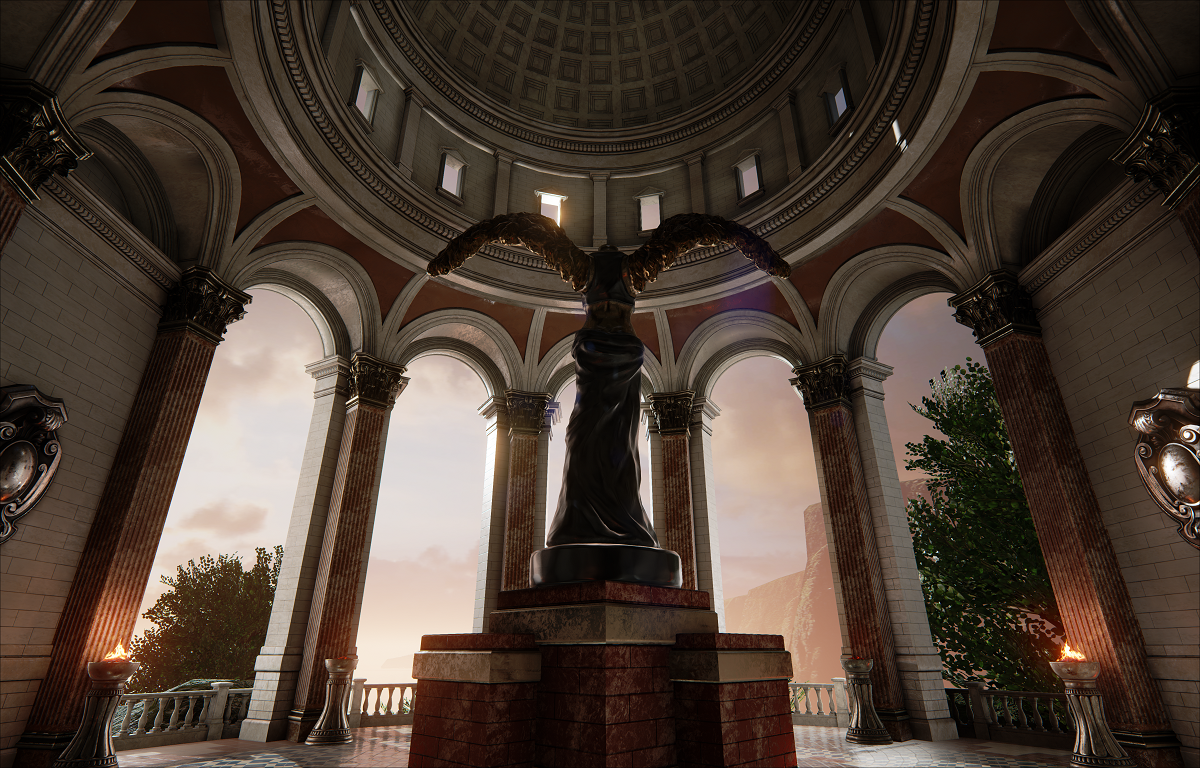
\includegraphics[width=0.45\textwidth]{images/lightoff.png}

            
\includegraphics[width=0.45\textwidth]{images/landscapeOn.png}
            
\includegraphics[width=0.45\textwidth]{images/landscapeOff.png}
            
            \caption{Sample screenshot of the test scenes (top Temple, bottom Mountainous), with DoF enabled (left) and disabled (right).}
            \label{fig:temple1}
\end{figure*}


%%%%%%%%%%%%%%%%%%%%%%%%%%%%%%%%%%%%%%%%%%%%%%%%%%%%%%%%%%%%%%%%%%%%%%%%%% OLD
%Recent advances in hardware technology have led to consumer level HMDs such as Oculus Rift \cite{oculusDK1}, ideal for immersive visualistion of virtual reality (VR) as a personal device. Support from openly-accessible Source Development Kit (SDK) software for the Oculus\cite{oculusSDK} has resulted in a growing ecosystem of games, movies, and VR applications. This, coupled with that high quality of the Oculus represents the first time VR has been so widely accessible in consumer market. \\

%Although HMDs are an ideal device to provide immersive stereovision in a wide range of field of view, the primary downside of HMDs is that people often report unpleasant reactions. These reactions, including symptoms such as headaches, nausea, dizziness and eyestrain\cite{howard:depthPerception} are often similar to those experienced by people who suffer from motion sickness, and are collectively termed \textbf{\textit{simulator sickness}} \cite{mccauley}. \cite{virtual:expect} indicates that as many as 80\% of people experience adverse effects when using HMDs. \\

%The human visual system uses a number of cues to infer depth and distance. Foremost among these cues are accommodation, the flexion of the lens in the eye required to form a focused image, and vergence, the rotation of the eyes to form a single, binocular image. In stereo displays, these two cues do not match: the eye accommodates to the physical screen in the screen, while the eyes converge towards a variety of depths, depending on the virtual depth of the observed object in the stereo scopic scene \cite{rushton99}. This leads to a conflict in the user's ocular system, which is known to be a cause of visual discomfort \cite{shibata:zone}. \cite{kim14} shows that in stereo 3D viewing, when the accommodative demand is fixed (as is the case for a HDM) and the vergence demand changes, a greater rate of change of the vergence demand results in a higher visual discomfort, a major contributing factors to Simulator Sickness, and as such mitigating this conflict is the main challenges to reduce visual discomfort in stereo scopic displays including HMDs. \\

%\cite{moss08} reported that modification to HMD hardware design are required to reduce Simulator Sickness, and Lanman and Luebke \cite{Lanman13} adapted light field displays to their HMD prototype for mitigating the problem. Although it shows a promising result, it still has many practical limitations such as display resolution and pixel pitches. Recently, \cite{Duchowski:2014:RVD:2628257.2628259} showed their perceptual test results reporting that gaze-contingent DOF can reduce the visual discomfort when viewing in stereoscopic display using LCD monitors arranged in haploscope. They used an external eye-tracker to provide pixel-accurate eye-tracking in their experiment. Such extra setup is intrusive in psychophysical test of consumer level devices.\\

% What is our solutions and contribution
%In this paper, we perceptually evaluate human visual system to show effectiveness of dynamic DOF blur to mitigate the visual discomfort when viewing in stereoscopic HMDs. As we know, this is the first experimental report to evaluate effectiveness of dynamic DOF blur in HMDs. Our test system can be realized without any hardware modification or external intrusive devices, as it only relies on positional data already captured by the Oculus. We implemented dynamic DOF \cite{dx9:dof} in Unreal Engine 4\cite{unreal} and performed a series of psychophysical test to show the effectiveness of dynamic DOF blur in Oculus, using participant responses to questionnaire \cite{ssq} on discomfort symptoms as a metric. On average, we showed a reduction of visual discomfort occurs when using dynamic DOF blur on HMD. Since our experimental setup does not require extra device or hardware modification, the result can be simply adapted in many applicatios viewed in general stereoscopic HMDs.


%%%%%%%%%%%%%%%%%%%%%%%%%%%%%%%%%%%%%%%%%%%%%%%%%%%%%%%%%%%%%%%%%%%%%%%%%% OLDEST
% The recent advances in hardware technologies release of the Oculus Rift DK1 (hereafter referred to as the Oculus) Development Kit brings, Virtual Reality (VR) technology to market at a price point (<\$400) suitable for reasonable consumer access. Support from companies such as Valve, who have released patches to popular games such as Half Life 2 and Team Fortress 2 to enable VR viewing modes, along with the availability of the openly-accessible SDK for the Oculus has resulted in a growing ecosystem of games, movies and applications designed with VR capabilities. This, coupled with that high quality of the Oculus represents the first time VR has been so widely accessible: prior VR implementations such as the Nintendo VirtualBoy or Vuzix VFX-1 suffered from poor execution and an extremely limited range of usable applications. \\

% The majority of VR implementations rely on a 3D stereoscopic display (S3D), in which each of a user's eyes are shown slightly differing images to simulate natural vision. This allows the VR device to provide a more immersive experience than traditional 2D display methods. Devices in which this S3D display is mounted to the user's head, instead of being placed in a fixed location like a traditional LCD computer screen are referred to as binocular Head Mounted Displays (HMDs), and are known to have several advantages, foremost of which is the screen's proximity to the user in a HMD occluding external visual stimuli, allowing the user to focus exclusively on the content shown on the S3D screen. Other varieties of HMD exist, including those that present an identical image to each eye (biocular) and those that only present one image (monocular), however we only focus on binocular HMDs. \\

% The primary downside of HMDs is that people often report unpleasant reactions to HMD systems. These reactions, including symptoms such as headaches, nausea, dizziness and eyestrain\cite{howard:depthPerception} are often similar to those experienced by people who suffer from Motion Sickness, and are collectively termed Simulator Sickness\cite{mccauley}. \cite{virtual:expect} indicates that as many as 80\% of people experience adverse effects when using HMDs. \\

% Given the rising popularity of consumer level VR, it is thus imperative that simulator sickness is  mitigated for the majority of vision-normal consumers to allow the continued growth of the applications.  The ideal solution for the current existence of a VR ecosystem should:\\
% \begin{itemize}
%	\item Be device agnostic. 
%	\item Require no purchase or installation of external devices to modify behaviour of current-market technologies. 
%	\item Allow application in both passive (such as film) and active (such as gaming) VR tasks. \\
%\end{itemize} 

%The current existence of a VR ecosystem where many separate developers are publishing VR ready content, and multiple VR devices (of which the Oculus is currently the most well known) exist, solutions for reducing Simulator Sickness optimally should:\\
%\begin{itemize}
%	\item Be device agnostic. 
%	\item Require no purchase or installation of external devices to modify behaviour of current-market technologies. 
%	\item Allow application in both passive (such as film) and active (such as gaming) VR tasks. \\
%\end{itemize} 

%Since HMDs display content at a very small distance from the viewers eyes ($<10cm$), something something low margin, extremes of vision.

% If any, what was the problems or limitations of the previous solutions ?
% These restrictions mean that prior implementations for reducing Simulator Sickness are insufficient. For example, \cite{Duchowski:2014:RVD:2628257.2628259} use a external eye-tracker to provide pixel-accurate eye-tracking in their solution, and \cite{moss2008characteristics} conclude that modification to HMD design and user behaviours are required to reduce Simulator Sickness. Furthermore, implementations that require eye tracking have to exclude users who are unable to calibrate the tracker properly, through either minor visual aberrations or unusual visual activity. \\


%%%%%%%%%%%%%%%%%%%%%%%%%%%%%%%%%%%%%%%%%%%%%%%%%%%%%%%%%%%%%%%%%%%%%%%%%% Summary and Contribution
% What is the proposed solution ? (overview of the methods)
% Adding in rationale for the method chosen. Not sure if this is the correct location or ot.
% The human visual system uses a number of cues to infer depth and distance. Foremost among these cues are Accommodation, the flexion of the lens in the eye required to form a focused image, and Vergence, the rotation of the eyes to form a single, binocular image. On HMDs, these two cues do not match: the eye accommodates to the physical screen in the HMD, ~6cm from the eye, while the eyes converge towards a variety of depths, depending on the virtual depth of the observed object in the S3D scene.\\

% Add an image here detailing the two, and how they conflict on the HMD

% This leads to a conflict in the user's ocular system, which is known to be a cause of visual discomfort \cite{shibata:zone}, a major contributing factors to Simulator Sickness, and as such we propose a system aimed at mitigating this conflict. \cite{Duchowski:2014:RVD:2628257.2628259} shows that blurred images (ie, images on the retina that either have failed to accommodate, or were artificially blurred) in the human visual system do not carry the same stimuli to fuse into a single binocular image as focused images do . 



